\documentclass[12pt,letterpaper]{article}

%\usepackage{times}
%\usepackage{epsfig}
\usepackage{graphicx}
%\usepackage{amsmath}
%\usepackage{amssymb}
\usepackage{hyperref}
\usepackage{tabularx}
\usepackage[left=1in, right=1in, top=1in, bottom=1in]{geometry}
\usepackage{titling}
\usepackage{setspace}
\usepackage{sectsty}
\usepackage{tabto}
\graphicspath{{../img/}} % adds the assets directory to the path, throw your images there
\usepackage{fancyhdr}
\pagestyle{fancy}
\fancyhf{}
\fancyheadoffset{0cm}
\renewcommand{\headrulewidth}{0pt} 
\renewcommand{\footrulewidth}{0pt}
\fancyhead[R]{\thepage}
\fancypagestyle{plain}{%
  \fancyhf{}%
  \fancyhead[R]{\thepage}%
}

\usepackage{cite}
\usepackage[sectionbib]{natbib}
\renewcommand{\refname}{}

\begin{document}
\fontfamily{ptm}\selectfont
\sectionfont{\fontsize{12}{12}\fontfamily{ptm}\selectfont}
\doublespacing
%%%%%%%%%%%%%%%%%%%%%%%%%%%%%% TITLE %%%%%%%%%%%%%%%%%%%%%%%%%%%%%%%%%%%%%%
\setlength{\droptitle}{1in} 

\title{\large{AN ABSTRACTED PYTHON CLASS FOR TDSP ML PROJECTS: \\ EXAMPLE USE CASE WITH WINE ID \\\vspace{1.2in}}}

\author{
Kevin Geidel \\
MSDS 422: Practical Machine Learning \\
Northwestern University \\
June 2, 2024 \\
}

\date{}
\maketitle
\thispagestyle{empty}	
\clearpage
\setcounter{page}{1}

%%%%%%%%%%%%%%%%%%%%%%%%%%%%%% PAGE 1 %%%%%%%%%%%%%%%%%%%%%%%%%%%%%%%%%%%%
\section{Executive summary}
\tab Given the rising preveleance of data science teams in industry and the widespread adoption of the \emph{Team Data Science Process (TDSP)} methodology, an abstracted library that streamlines common TDSP projects would allow ``citizen developers'' in data related roles to increase the efficiency and performance of their \emph{Machine Learning (ML)} applications. There are commerical data science solutions available for purchase. However, many small teams are using agile project management, cloud computing resources and versitile opensource frameworks to create low cost, high performaning analytics and data science tools that are tailor made for many different settings throughout various enterprises \citep{Hyatt:2024}.

The proposed \texttt{Python} classes create a work flow that mirrors the TDSP \citep{tdsp:2024}. 
Various stages in the TDSP (which is illustrated in figure \ref{fig:tdsp}) are represented by data models and have methods for applying standard work to these structures, moving them along the path to the next stage.
The benefits of using customized libraries to conduct ML projects are shortened development cycles, more robust/stable applications, greater interoperability amongst team members and more time to focus on making models that perform better and provide more actionable conclusions. The code for the project (and this paper) can be found in the \texttt{GitHub} repositiory located at \url{https://github.com/kgeidel/MSDS-422-final-project} \citep{GeidelRepo:2024}.

The concept is explored with a use case that seeks to deploy a binary classifier for a defect prediction application. Using the \texttt{wine} dataset \citep{Vanschoren:2014} from \texttt{openml.org} we have 14 features for 178 records that include labels on if the sameple is wine or not. \emph{Exploratory Data Analysis (EDA)} is conducted with the aim of selecting, training and tuning four models to classify, for now, a sample as wine or not. This would be extended to a model that seeks to predict samples that run a high probability of being defective or non-conforming. Emphasis is on turning this wine classifier deployment into a DRY (\emph{Don't Repeat Yourself}), generic (but still flexible) and easy to deploy tool that data scientists can use to expedidate routine data exploration, data wrangling and datamining. 


\section{Research design}
\tab 
-Can we abstract datamining to automate model evaluation and selection?
-In a big MS thesis like data sync design where you use ORM youll want a custom pipeline toolkit 
-Wine defect prediction use case   

\section{Exploratory Data Analysis (EDA)}
\tab 

\section{Datamining data models}

\section{Data pipeline and ML preprocessing}
\tab 

\section{ML engineering, evaluation and deployment}
\tab 
- data transformations!

\section{Findings}
\tab 

\section{Conclusions}
\tab 


\pagebreak
\section*{\center{Appendix}}


\begin{figure}[h!]
  \centering
    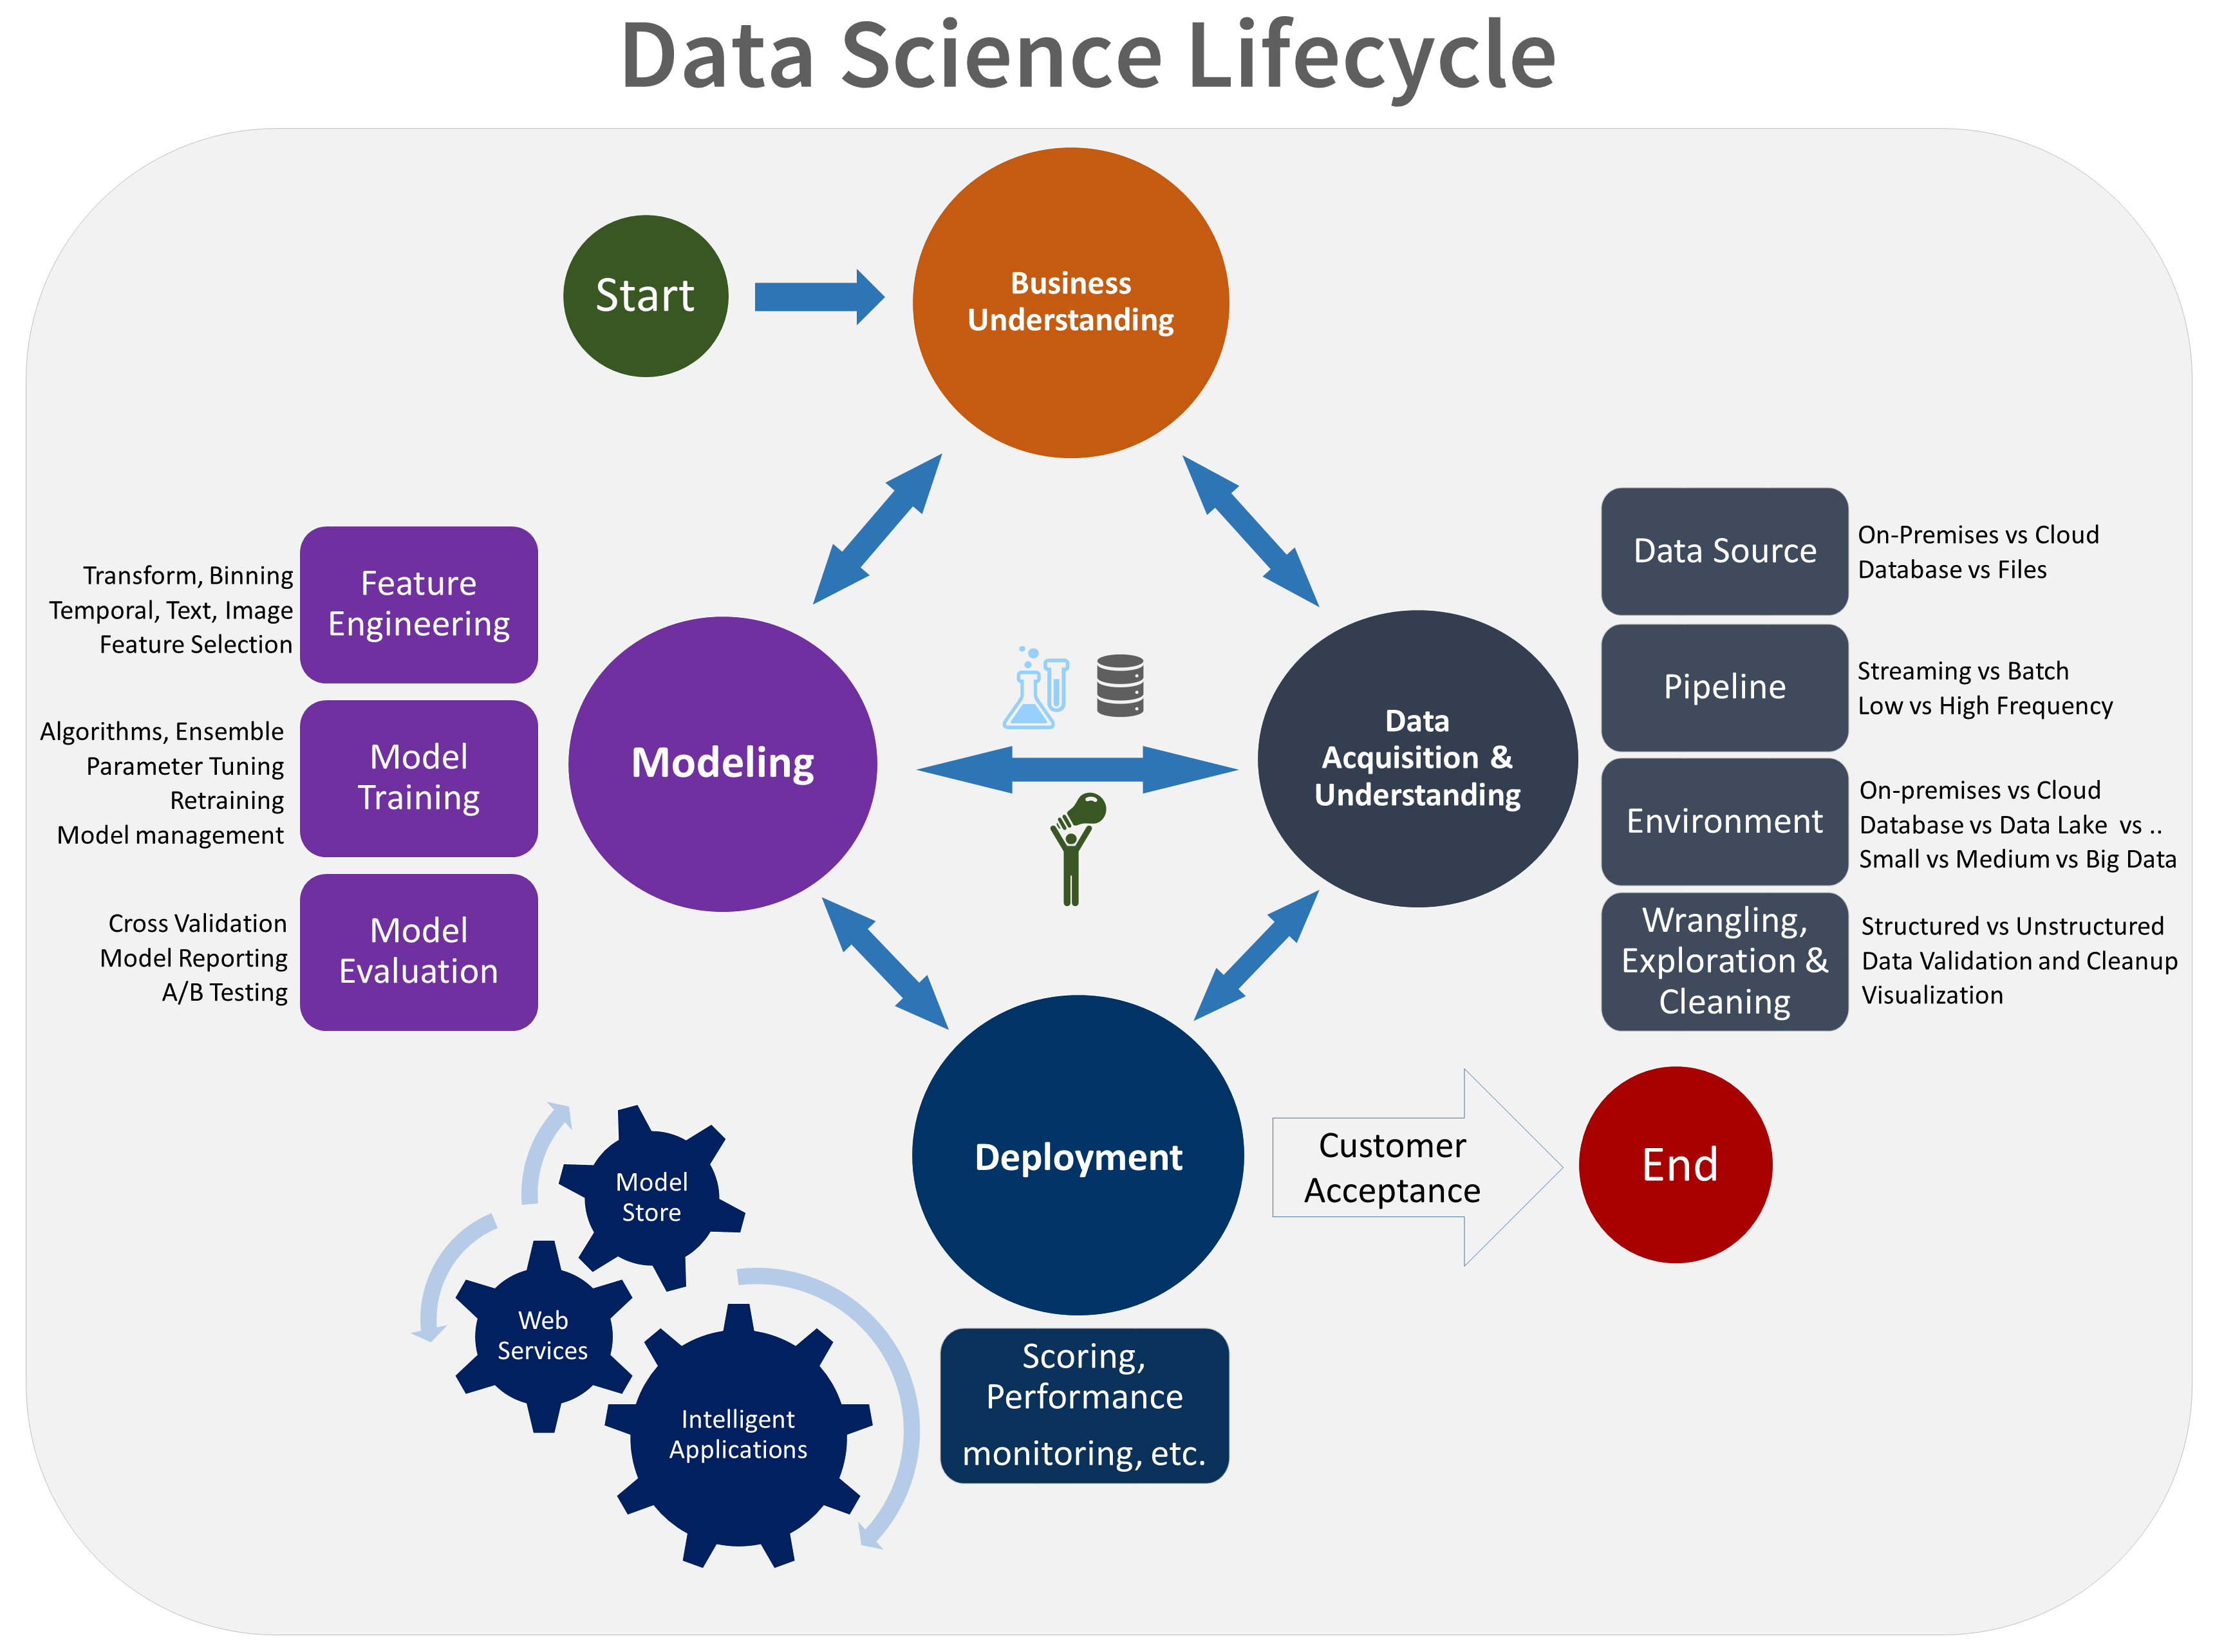
\includegraphics[width=1.0\linewidth]{../img/TDSP_Data_Science_Lifecycle.png}
    \caption{(color online) The ``data lifecycle'' in Team Data Science Process (TDSP)}
    \label{fig:tdsp}
  \end{figure}


\clearpage
\section*{\center{References}}
\bibliographystyle{chicago}
\center{\bibliography{references}}



\end{document}